\section*{Abstract}

This thesis explores the design and implementation of a \acrfull{dt} for a green smart home, integrating \acrfull{eud} with \acrfull{ml} algorithms. \acrshort{eud} approaches enable users to control and manage their \acrfull{iot} environments, e.g.\ through trigger-action routines. The \acrshort{dt} enhances energy consumption awareness by allowing users to monitor the energy consumption of smart appliances and simulate scenarios related to the creation of routines. These simulations assess the effects of appliance activation involved in the routines and potentially modify them to save energy based on the \acrshort{dt}'s suggestions.

An hypothetical home was designed as a starting point for the creation of the \acrshort{dt}. A number of appliance types were chosen to be introduced into the home, based on their commonality in European households and their availability in the 
The appliances were extracted from the GREEND\footnote{\url{https://www.andreatonello.com/greend-energy-metering-data-set/}}~\parencite{monacchiGREENDEnergyConsumption2014} and UK-DALE\footnote{\url{https://jack-kelly.com/data/}}~\parencite{kellyUKDALEDatasetDomestic2015} datasets, which were selected through a scoping review among other power consumption datasets available in the literature, prioritizing those with a large number of appliances gathered in European households. This is significant to minimize geographic variations in appliance usage patterns and to produce results that are relevant for Italian households.

The selected datasets however do not record the operation mode of appliances at a given time. For example, a washing machine could be in a certain wash program at a given time. This information is required to assign a specific energy consumption value to the operation modes and to estimate their duration. This limitation is overcome using an approach inspired by~\cite{castangiaClusteringApplianceOperation2023}, which uses unsupervised deep learning techniques to cluster appliance operation modes from a learned, latent state representation of the raw data. Figure~\ref{fig:high-level-procedure} illustrates the main steps of the approach. First, a segmentation procedure is applied
to the raw appliance data to identify the active states that contain the actual power signatures of the device. These signatures are then standardized and fed to a deep autoencoder model, which learns to reconstruct the operation cycles and encode them into a latent representation. Next, a K-means clustering algorithm is applied to the
latent representation, to group the operation cycles into different programs of the device. Finally, the clusters are mapped to the operation modes of the appliance.

\begin{figure}
    \centering
    
\includegraphics[width=.8\linewidth]{images/high_level_procedure.png}
    \caption{High level procedure for identifying the operation modes of appliances}
    \label{fig:high-level-procedure}
\end{figure}

The operation modes are used by a \acrfull{rest} \acrfull{api}, which exposes endpoints for accessing and manipulating the data and
routines of the smart home, displaying the energy consumption of the appliances over time, and simulating the effects of adding new routines and resolving potential conflicts with the existing ones. The \acrshort{api} separates the \acrshort{dt} logic from the user interface, enabling the \acrshort{dt} to be integrated with various clients, such as the web application developed in this thesis to demonstrate the functionalities of the \acrshort{dt}.

The \acrshort{dt} creates a state matrix of the appliances throughout the day, based on the defined routines. The state matrix tracks the operation mode of each appliance for every minute of the day. It is used to evaluate the conflict scenarios and to simulate the addition of a new routine. Figure~\ref{fig:state-matrix} shows an example of a state matrix, which displays the operation modes of the appliances in the hypothetical home throughout the day, using a predefined set of routines.

\begin{figure}
    \centering
    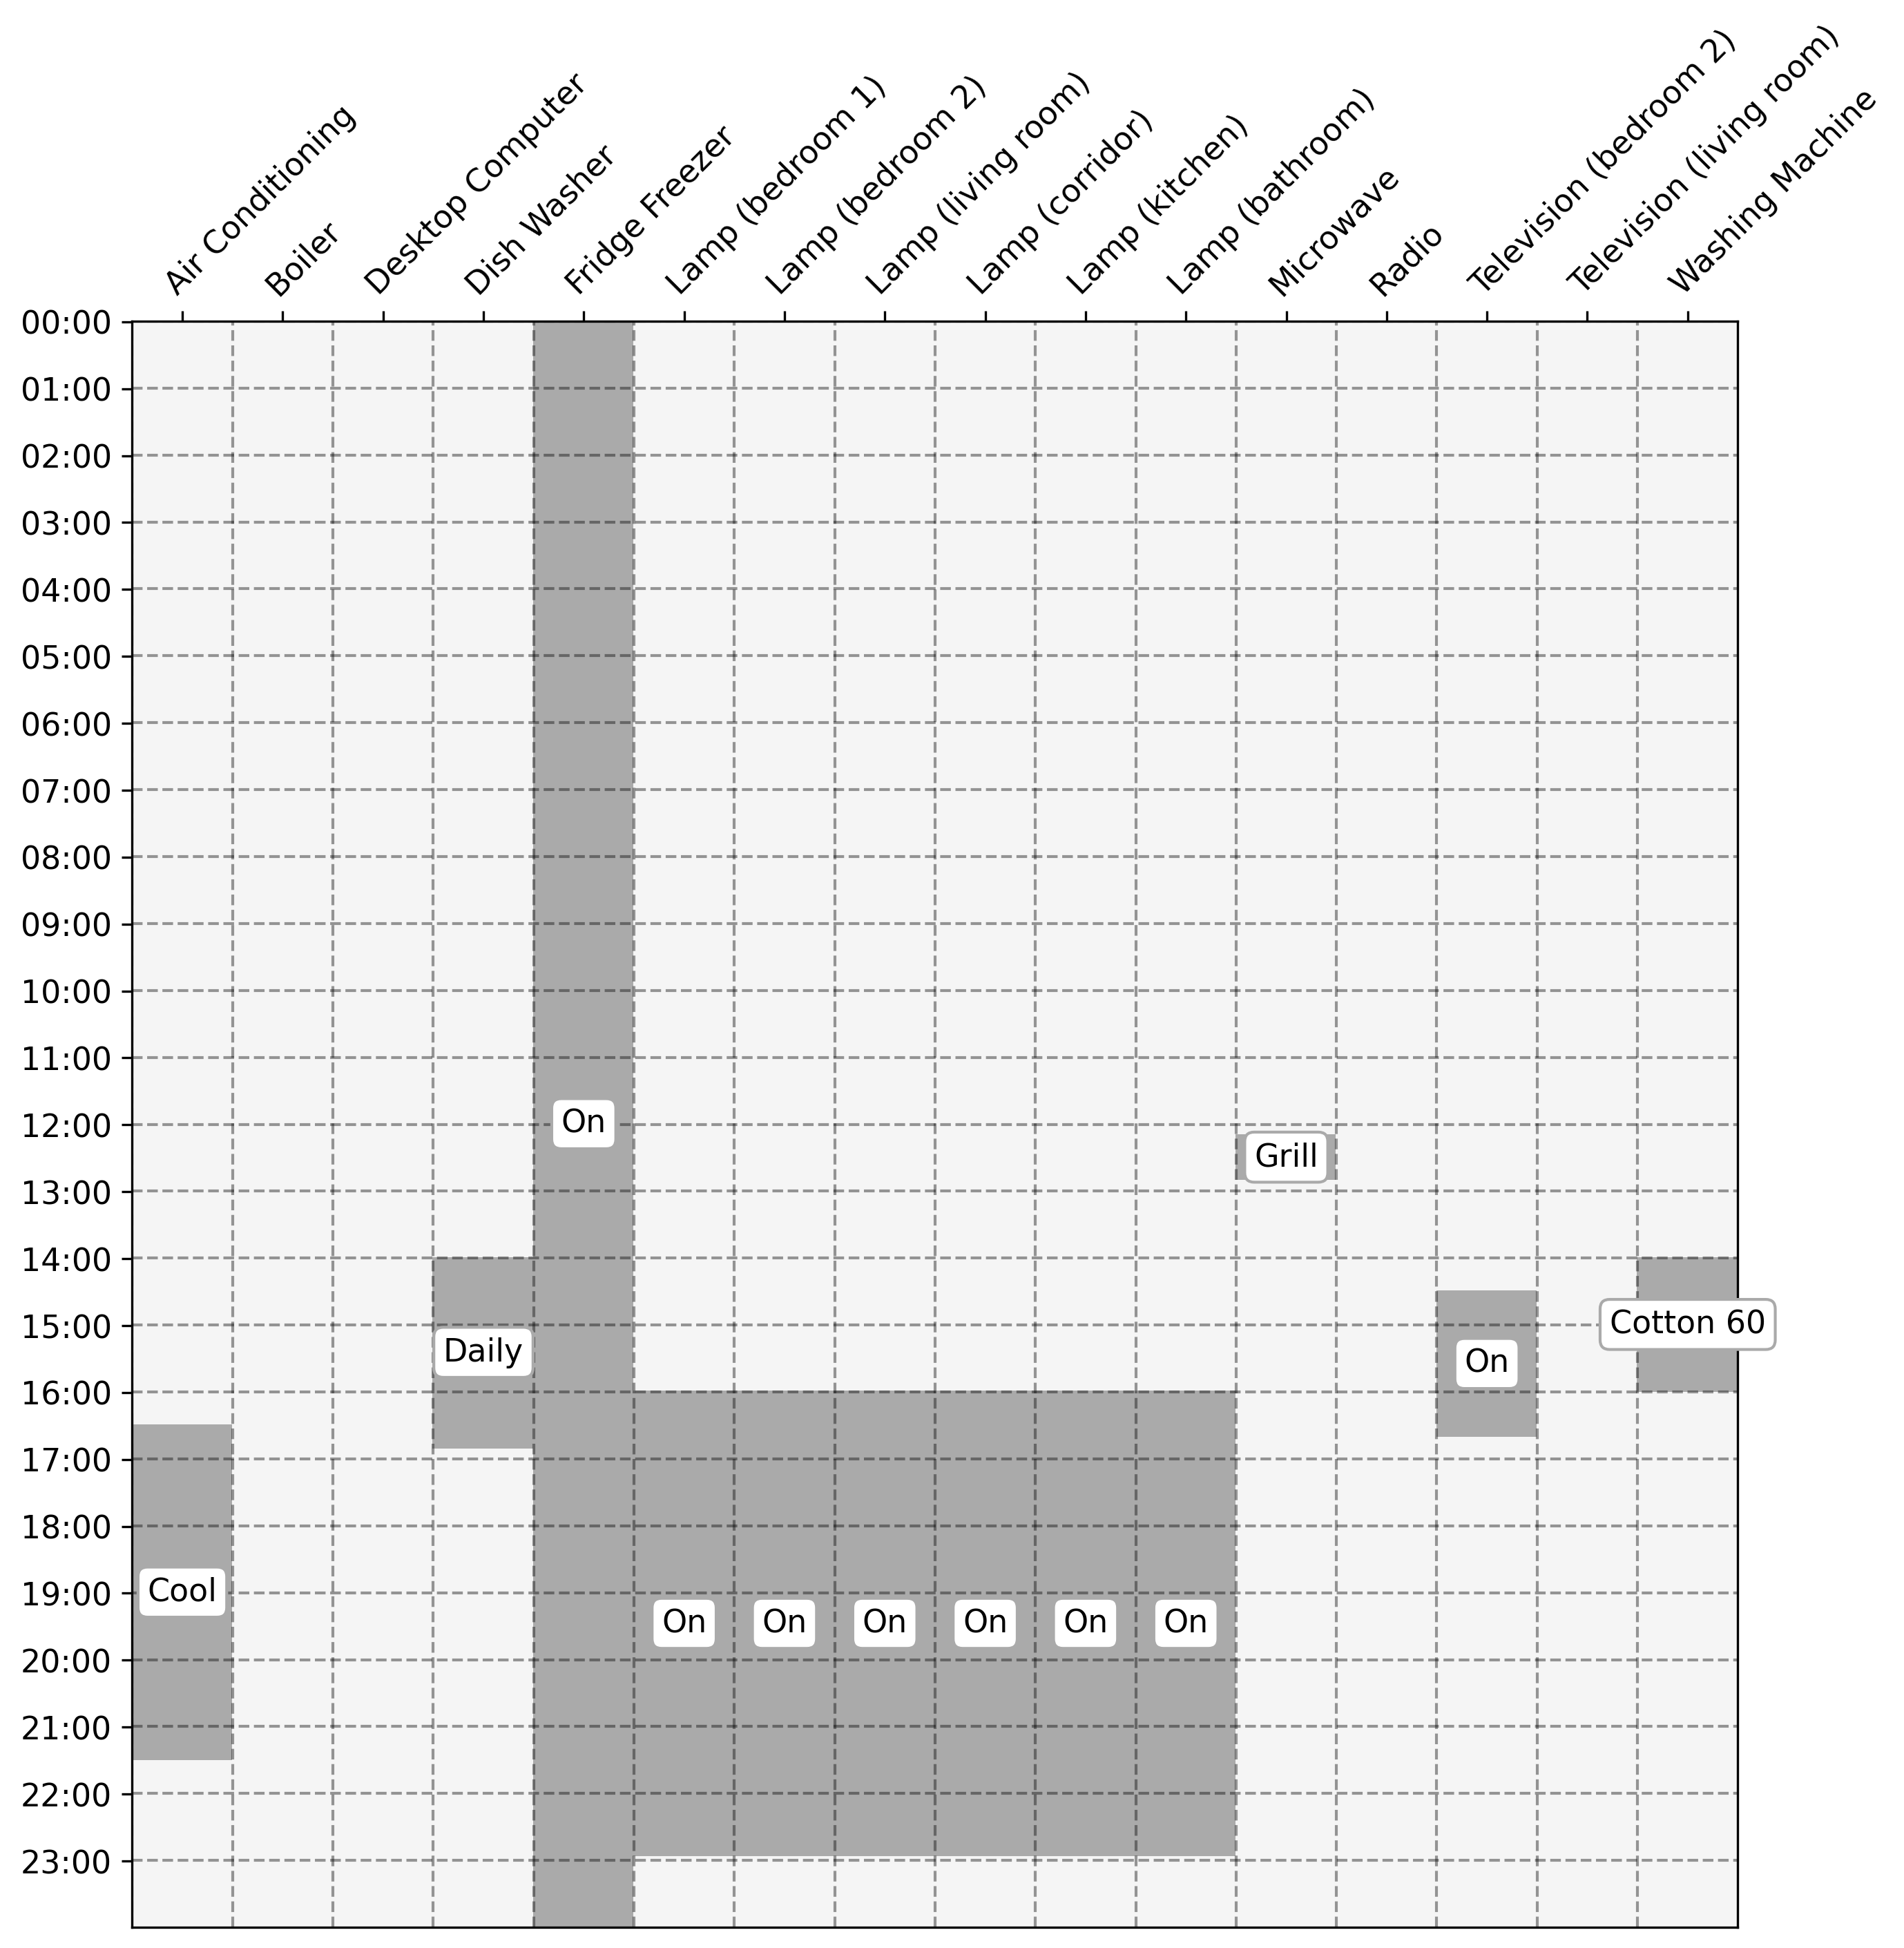
\includegraphics[width=.5\linewidth]{images/real_matrix.png}
    \caption{Example of a state matrix}
    \label{fig:state-matrix}
\end{figure}

When a user would like to create a new automation
to manage their appliances, the DT allows the user to simulate what
would happen in case of its activation, by returning different types
of feedback associated with different scenarios:

\begin{itemize}
    \item  Conflict that determines overcoming the energy meter load capacity: in this case the automation can not be executed as-is because it includes an appliance activation that will bring energy consumption of all active automations over the admitted load capacity for the energy meter (in Italy it is commonly set to 3kWH for domestic use). The DT may suggest how the automation could be modified, for example, its activation could be postponed after an appliance involved in another automation has completed its operation;
    \item Conflict due to operation mode inconsistency: this case occurs whenever the automation under creation includes the activation of an appliance in a given operation mode (e.g., for a washing machine, a short sports cycle), but there is another automation scheduled on the same appliance with a different operation mode in an overlapping time slot. The DT may present the user with different options: the deletion of one of the two conflicting automations or the modification of one of them;
    \item No conflict, but a suggestion to be more sustainable: in this case, even if the automation can be executed without generating conflicts with other automations, the DT may suggest reducing energy consumption costs, avoiding cases of non-sustainable appliance activation.
\end{itemize}

This research is significant as it contributes to the development of a new paradigm for smart and sustainable living, and advances both theoretical and practical knowledge of \acrshort{dt}s in the building sector.